\newpage
\thispagestyle{sectioned}
\chapter{Migración de SwellRT a Android}

	En esta parte de la memoria se hablará de los aspectos más destacados del proceso de migración de la tecnología de colaboración en tiempo real presente en SwellRT, basada en el protocolo Wave (ver Sección \ref{ssec:wave}), a Android. Para ello se identificará el objetivo de esta parte del proyecto y se detallarán los problemas encontrados y cómo se solucionaron. Al final se discutirá el resultado obtenido. 

  \section{Objetivo} \label{sec:migration}
  
    El framework de SwellRT utiliza un servidor WIAB y el protocolo Wave, ambos desarrollados en Java/GWT. El \textbf{SDK de Android} \cite{ref:android_sdk} es compatible con Java, así que a priori la implantación del servidor no supone problemas en los dispositivos móviles. Sin embargo, existe un problema con el API de SwellRT, ya que el lado del cliente fue desarrollado en Javascript usando el framework GWT. Android no soporta de forma nativa estas tecnologías, así que es necesario estudiar el código de SwellRT para sustituir todo el código que haga uso de Javascript/GWT por código compatible con Android. 
    
    No obstante, al principio hubo ciertas dificultades relacionadas con la integración del código de SwellRT original en el entorno de desarrollo de Android. 
    
    
    \textbf{El objetivo de esta parte del proyecto es conseguir que un cliente desplegado en Android sea capaz de conectarse e interactuar con un servidor Wave/SwellRT sin problemas para hacer uso de sus características.}  

	\subsection{Migración: Identificación y Solución de Problemas}	
	
	\textbf{Resumen}:
	
	\begin{itemize}
	  \item Migrando la Conexión HTTP a Android \ref{sssec:conHttp}.
	  \item Migrando la Conexión WebSocket a Android \ref{sssec:conWave}.
	  \item Migrando el Logging a Android \ref{sssec:conFinAndLogin}.
	  \item Creando el Servicio Android \ref{sssec:orgCodServAnd}.
	\end{itemize}
	
	El objetivo de esta parte del proyecto es conseguir que el cliente de SwellRT se pueda desplegar en Android para así conseguir que se conecte al servidor Wave In a Box (Ver sección \ref{sssec:wiab}) que también incluye. Para ello lo primero que se hará será desplegar el servidor en el ordenador clonando el repositorio de GitHub \cite{ref:swellRT_github} de SwellRT y siguiendo los pasos descritos en el Readme del proyecto. Para comprobar que el servidor se ha instalado correctamente, se puede ejecutar por consola (ver Readme) y abrir un navegador Web con la dirección http://localhost:9898. Se crea entonces un usuario y contraseña de prueba. Este paso es importante ya que la aplicación Android intentará conectarse contra este servidor mientras estemos haciendo pruebas de desarrollo. 
	  
	  A continuación se crea un proyecto Android en Eclipse y se incluyen en él todas las clases de SwellRT. Uno de los componentes principales de Android a la hora de desarrollar en esta plataforma son las \textbf{Actividades} \cite{ref:android_activities}, que representan las pantallas que se le muestran al usuario y que responden a su interacción programáticamente. Por tanto, se crea una nueva actividad  principal (waveAndroid.java) que se ejecutará al lanzar la aplicación y que por el momento intentará conectarse al servidor especificando por código el usuario y contraseña que hemos creado antes en el servidor. SwellRT realiza este login contra el servidor usando dos tecnologias: HTTP \cite{ref:http_authentication} y WebSockets \cite{ref:webSocket_ref}.
	  
  
    		\subsubsection{Conexión HTTP}\label{sssec:conHttp}
	
	Wave fue desarrollado para utilizar el protocolo WebSocket para la conexión al servidor, pero esta tecnología necesita realizar una autenticación HTTP previa llamada ''handshake''. Lo primero que se hará será otorgar \textbf{permisos de conexión a internet} a la aplicación. Android utiliza un \textbf{sistema de permisos} \cite{ref:android_permissions} para controlar los privilegios de cada aplicación. Estos permisos se declaran en el \textbf{Manifiesto} de la aplicación \cite{ref:android_manifest}, archivo que declara sus características. Para ello basta con añadir lo siguiente al manifest.xml de la aplicación:
	  
	  \lstset{language=XML, breaklines=true, autogobble=true, basicstyle=\ttfamily\footnotesize}
	  \begin{lstlisting}[frame=single]
	  	<uses-permission android:name="android.permission.INTERNET"/>
	  \end{lstlisting}
	  
	  	 También hay que tener en cuenta que cuando estamos en el emulador no estamos en la misma red que el ordenador en el que trabajamos, por lo que la conexión a la URL http://localhost:9898 no es válida. No obstante, esto tiene facil solución pues \textbf{el emulador de Android define unas direcciones IP de red especiales} \cite{ref:android_netAddress} para este tipo de casos. Basta con sustituir localhost por la direccion 10.0.2.2 para conseguir acceder al servidor WIAB desplegado en el ordenador. La dirección URL sera por tanto: \textbf{http://10.0.2.2:9898}. 
	  
	 Lo siguiente que se hará será ejecutar el código de Login del cliente SwellRT para intentar localizar dónde se lleva a cabo la conexion HTTP. Para ello se llama desde la actividad principal (WaveAndroid.java) al método startSession() de la clase WaveClient.java pasándole el usuario y la contraseña antes creados.
 
	 Esto provoca un error de ejecución y la aplicación se cierra. Lo siguiente que hacemos es depurar la aplicación (Ver Seccion \ref{sssec:debug}) estudiando el LogCat \cite{ref:android_logcat} (Ver Figura \ref{fig:android_logcat}) para ver dónde se produce el error. Se descubre que el problema esta localizado en el método login() de la misma clase, que intentaba realizar una \textbf{petición POST HTTP} al servidor utilizando un \textbf{RequestBuilder} de la librería \textbf{com.google.gwt.http.client}. He aquí el primer problema: la actual conexión utiliza métodos de GWT/Javascript para hacer la petición Post y Android no es compatible con esta tecnología.   
	 
	\begin{figure}[H]
      \centering
	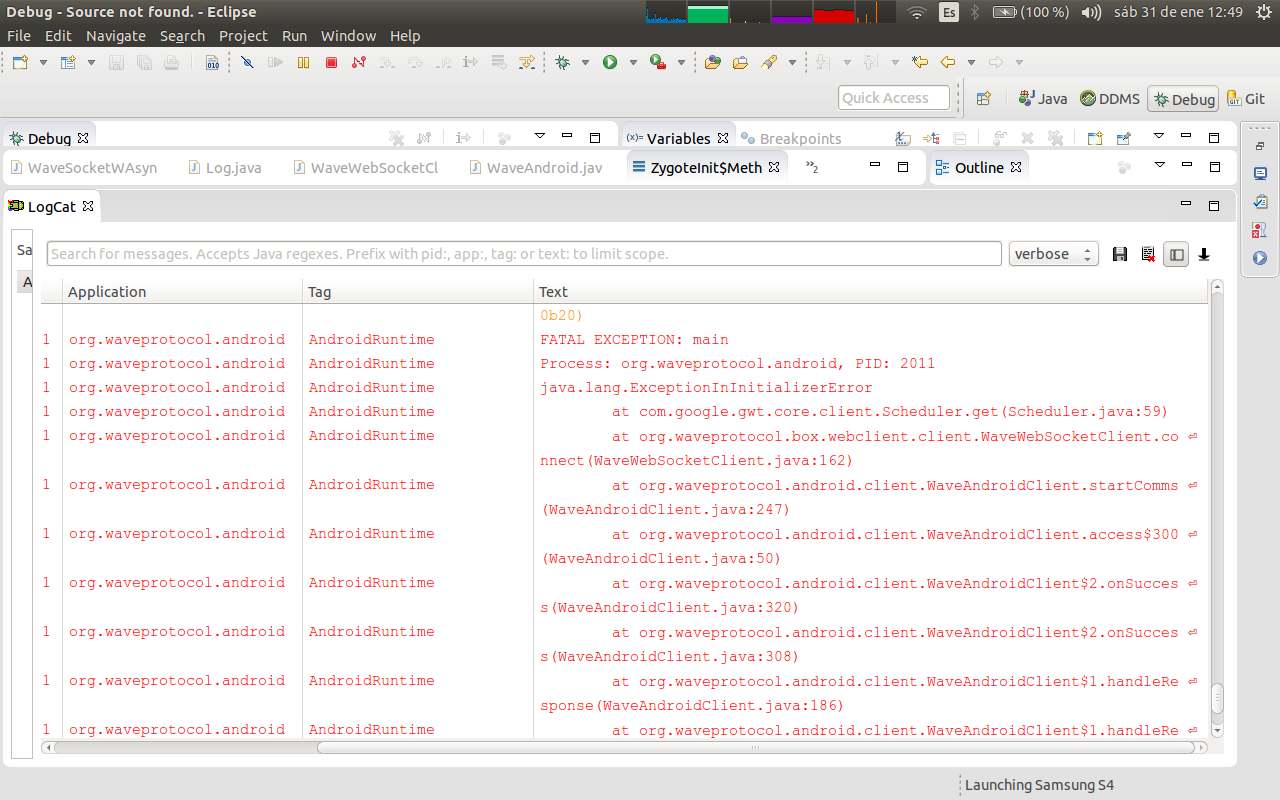
\includegraphics[keepaspectratio, scale=0.3]{Media/Captures/logcat_example.png}
      \caption{Ejemplo de Traza de Error en Logcat}
      \label{fig:android_logcat}
    \end{figure} 
	 
	 Hay por tanto que encontrar una librería similar compatible con Android que construya una petición \textbf{HTTP POST} y la envíe al servidor. La primera opción que sse valoró fue utilizar la \textbf{librería HTTP Apache} \cite{ref:apache_http}, incluida en el SDK de Android desde sus primeras versiones. Sin embargo, Google recomienda \cite{ref:http_recommmendations} a partir del API 10 (Android 2.3 "Gingerbread") utilizar la \textbf{librería HttpURLConnection}\cite{ref:android_httpUrlConnection}, también incluida en el API. Por tanto esta última es la que se elige para la migración. 
	 
	 Se puede ver un esquema simplificado de la nueva estructura del login HTTP en la Sección \ref{ssec:codeHTTP} del Apéndíce.
	  
	 Sin embargo, aquí no acaba el problema. Por cuestiones de usabilidad y de respuesta a la interacción del usuario, Android establece dos reglas para trabajar con el proceso de la actividad que se le esta mostrando al usuario (llamado \textbf{UI Thread}) \cite{ref:android_processes}:
	  
	  \begin{itemize}
	  	\item \textbf{1. No bloquear el UI Thread}
	  	\item \textbf{2. No acceder al UI Thread directamente desde otro Thread}
	  \end{itemize}
	  
	  La conexión a un servidor es un proceso susceptible de durar un tiempo variable según las condiciones de la red, lo cual deja la aplicación en espera hasta que se realiza dicha conexión,  bloqueando el UI Thread. Por tanto, se decidió usar un hilo (Thread) por separado en forma de \textbf{AsyncTask} \cite{ref:android_asynctask} para llevar a cabo la tarea de Login, tal y como recomienda Google hacer para trabajar con conexiones a la red \cite{ref:android_networking}. La ventaja por tanto de usar otro hilo para esto es que la actividad principal no se bloquea.
	  	 
	  Es importante también destacar que la arquitectura de SwellRT y de Wave está planteada de manera que utiliza llamadas asíncronas (callbacks) para notificar al resto de la aplicacion del resultado de los procesos de conexión al servidor, por lo que el AsyncTask tendrá que usar el callback apropiado para notificar del éxito o fracaso de la conexión Http.
	 
	  Se puede ver un esquema del AsyncTask encargado del Login en la Sección \ref{ssec:codeAsynctask} del Apéndíce.
	    
	  Este proceso de conexión Http deberá devolver una Cookie que se tratará con el objetivo de generar un SessionId que será necesario para seguir con la conexión al servidor. \textbf{Llegados a este punto, se tiene un proceso de login Http que hace uso de la librería HttpUrlConnection y de un AsyncTask para realizar esa primera conexión al servidor.} Se depura la aplicación y se comprueba que efectivamente el login Http se realiza correctamente (la respuesta del servidor tiene código 200). \textbf{Sin embargo la aplicación aún no funciona correctamente, pues se cierra al intentar ejecutar el código que se encarga del siguiente paso de la conexión: conectarse por WebSocket.}    
    
    		\subsubsection{Conexión WebSocket}\label{sssec:conWave}
    
    Para realizar una conexión con el servidor Wave es necesaria una conexión mediante WebSockets\cite{ref:webSocket_ref}, tecnología que permite conexiones bidireccionales y asíncronas entre el servidor y el cliente (recordemos que la conexión en el modelo cliente-servidor tradicional está definida como unidireccional de cliente a servidor), de manera que cualquiera de los dos puede iniciar una conexión con el otro en cualquier momento e intercambiar información con éste. En el caso del protocolo Wave este comportamiento es el deseable, ya que al tratarse de un protocolo de comunicaciones federado en el que cualquiera en la red puede ser cliente o servidor, es importante que la conexión sea bidireccional. Además la asincronía es necesaria ya que, para mantener la consistencia en tiempo real \ref{sssec:realTime}, hace falta que el servidor que contiene las waves pueda iniciar una conexión con los clientes para notificar los cambios que se produzcan en dichas waves. Por tanto, el cliente Android debe ahora establecer una conexión WebSocket con el servidor WIAB. 
    
    La metodología a utilizar será la misma que para la conexión HTTP, se ejecutará el código de SwellRT para identificar dónde falla y por tanto cómo está estructurada la creación y gestión de WebSockets en la versión GWT.
    
    El cliente SwellRT original realiza esta conexión utilizando una librería llamada Atmosphere \cite{ref:atmosphere}, que proporciona un framework para Java que permite gestionar conexiones WebSocket junto a la conexión HTTP que subyace por debajo. Sin embargo, esta librería se encarga solo de gestionar la conexión, no de crear el WebSocket propiamente dicho. En el caso de SwellRT este WebSocket se crea utilizando la implementación que proporciona GWT llamada también WebSocket (WebSocket.java). Esta clase define las funciones básicas que debería tener el nuevo WebSocket: \textbf{onOpen()} para establecer la conexión, \textbf{onMessage()} para recibir mensajes por el WebSocket, \textbf{send()} para enviar mensajes y \textbf{onClose()} para cerrar la conexión. Asímismo el Websocket deberá también implementar una serie de callbacks (definidos en la interfaz WebSocketCallback.java) para notificar a la aplicación de la llegada de estos eventos del servidor. Los callbacks son: \textbf{onConnect()}, \textbf{onDisconnect()} y \textbf{onMessage(message)} respectivamente.
	
	Este WebSocket se crea utilizando un \textbf{patrón de diseño Factory}, que abstrae la creación de un objeto de su implementación, de manera que el desarrollador tenga acceso al objeto sin tener que preocuparse de cómo este implementado el WebSocket por debajo (ver WaveSocketFactory.java en SwellRT). En este caso, como ya se ha dicho, con Atmosphere y WebSocket GWT. No obstante, la aplicación no funciona tal y como está hecho en SwellRT ya que Android no soporta GWT de forma nativa. Hay que sustituir este código buscando una librería de Software libre que implemente un WebSocket en Android sobre Atmosphere y que porporcione las mismas funciones básicas descritas en el párrafo anterior.
	
	La solución encontrada fue utilizar \textbf{wAsync}\cite{ref:wAsync_github}, librería proporcionada por Atmosphere para trabajar con Websockets en Node.js, Java y Android. wAsync trabaja creando un socket que responde a eventos diversos, estando entre ellos eventos similares a los utilizados por la versión GWT de SwellRT: \textbf{on(EVENT.name())}, siendo EVENT el nombre del evento al que debe responder. 
	
	Se puede ver un ejemplo sencillo de utilización de wAsync en la Sección \ref{ssec:codewAsync} del Apéndíce.
	
	Como la arquitectura Wave utilizaba el patrón factoría, fue necesario sustituir la clase de WebSocket GWT por una de nueva creación llamada \textbf{WaveSocketWAsync.java}\cite{ref:wave_migration_github} que implementa los métodos de creación y configuración de un Websocket y de callback antes descritos. Asimismo se modificó la clase WaveSocketFactory.java para hacer uso ahora de esta nueva implementación del WebSocket compatible con Android. 
	
	Sin embargo, se ejecutó esta nueva versión de código y se encontró que la librería WAsync incluye dependencias a código que no está presente en la propia librería y que es necesario para crear el cliente AsyncHTTPClient que gestiona la conexión HTTP que subyace por debajo del WebSocket. Concretamente hace falta utilizar un HTTPProvider compatible con Atmosphere, tal y como recomienda hacer wAsync en su wiki \cite{ref:httpProvider_wAsync}. Para ello basta con añadir al proyecto las librerias oportunas (Ver Tabla de Dependencias \ref{fig:dependencies_swellRT}) y configurar el cliente segun lo descrito en dicha wiki:
		
	\lstset{language=Java, breaklines=true, autogobble=true, basicstyle=\ttfamily\footnotesize, commentstyle=\color{OliveGreen}, keywordstyle=\color{MidnightBlue}}
	  \begin{lstlisting}[frame=single]	
	  AsyncHttpClientConfig ahcConfig = new AsyncHttpClientConfig.Builder().build();
	  AsyncHttpClient ahc = new AsyncHttpClient(new GrizzlyAsyncHttpProvider(ahcConfig));
	  \end{lstlisting}
      
      Ahora, al ejecutar la aplicación se comprueba que la conexión al servidor se produce correctamente. Para completar esta parte del proyecto solo falta pedir al usuario su user y password, ya que hasta ahora se habían especificado a mano en el propio código para realizar pruebas.
	    
    		\subsubsection{Conexión final y Logging}\label{sssec:conFinAndLogin}
    
    Para probar que la aplicación migrada es funcional y es capaz de utilizar las características nativas de Android se creará una pequeña y sencilla pantalla de Login que pedirá al usuario la dirección del servidor Wave, un usuario y una contraseña.
    
    En el diseño de aplicaciones Android el componente principal de una app es la Actividad, que se corresponde con la pantalla con la que interactúa el usuario. La interfaz gráfica se usuario (UI) de las pantallas se encuentra separada del código de la aplicación en ficheros XML de Layout\cite{ref:android_layout}. A una Actividad se le especifica cuál es su archivo de layout en su método onCreate(), responsable de la creación de la actividad y sus recursos. 
    
    Se crea una Actividad llamada WaveAndroid.java que haga uso del layout Main.xml, en el cual se incluyen tres cajas de texto (llamadas EditText en Android) para que el usuario introduzca los datos. Además se guarda una referencia a estas cajas de texto en la Actividad para poder acceder al texto introducido y pasárselo al método login de Wave que hemos migrado anteriormente.
    
    	\begin{figure}[H]
      \centering
	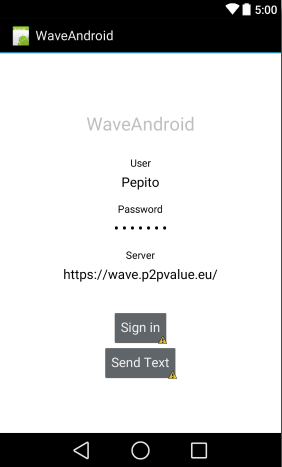
\includegraphics[keepaspectratio, scale=0.6]{Media/Captures/waveAndroidLogin.png}
      \caption{Pantalla de Login de WaveAndroid}
      \label{fig:android_waveLogin}
    \end{figure}
    
    Además fue necesario mejorar el sistema de mensajes de Log de la aplicación sustituyendo el framework de la librería SLF4J para Java usada por SwellRT por una versión más reciente desarrollada para Android\cite{ref:slf4j_android}. Esto se debió a que las librerías de las que hace uso wAsync utilizaban una versión más reciente de este logger.
        
    Por último se instaló la aplicación en el emulador o el dispositivo móvil y se probó que se mostraba la pantalla de login anterior. Se introdujeron los datos del servidor WIAB, de usuario y contraseña y comprobamos que se ha conseguido el objetivo de esta parte del proyecto: \textbf{el cliente Android realiza el login contra el servidor WIAB correctamente.} 
     
    		\subsubsection{Organización del código: Servicio Android}\label{sssec:orgCodServAnd}
    
    Una vez conseguida la conexión al servidor desde Android, se decidió revisar el código para intentar optimizarlo y organizarlo de manera que aprovechara mejor las características de Android y la arquitectura de Wave. Además, el API que permite gestionar el modelo de datos de SwellRT (Ver Sección \ref{sssec:swellRT}) está escrito en java, por lo que es plenamente funcional y compatible con el código de la migración a Android. A continuación se hablará de los motivos de dicha reorganización.
  
    Como ya se ha comentado anteriormente, el proceso de login se debe hacer en un hilo de ejecución separado del hilo principal o UI Thread, ya que Android no recomienda\cite{ref:android_processes} que tareas que tarden mucho tiempo en ejecutarse (cómo por ejemplo descarga de datos de la red) se ejecuten en el mismo hilo que la interfaz de usuario, pudiendo bloquear dicho hilo y obstaculizando por tanto la interacción del usuario con el dispositivo.
      
    Hasta ahora se había utilizado para ello una Actividad que cotenía el AsyncTask \cite{ref:android_asynctask} encargado de ejecutar el código de conexión al servidor en un hilo separado del UI Thread. Sin embargo, tal y como está definida la arquitectura de Wave y de SwellRT, la utilización de callbacks (ver secciones \ref{sssec:conHttp} y \ref{sssec:conWave}) es necesaria para notificar al resto de la aplicación de los eventos relacionados con el intercambio de datos con el servidor. Un AsyncTask ejecuta de una sola vez y de forma asíncrona el código que se le asigne a su método doInBackground(), de manera que una vez que termina su ejecución puede notificar el resultado de la conexión. Pero no queda a la espera de otros posibles eventos en el socket (como la recepción de mensajes o la desconexión). Es decir: \textbf{aunque se definan callbacks para esperar los eventos del servidor, el socket no podrá notificarlo porque no existe un hilo que quede a la espera de estos eventos.}

    Por otro lado, cada vez que se quisiera realizar algún tipo de interacción con el servidor habría que utilizar un AsyncTask específico para ello, lo cual no hace sino añadir más código a la aplicación. Otra desventaja de los AsyncTask en la implementación inicial es que si la Actividad que lo esta ejecutando pasa a segundo plano (por ejemplo si el usuario cambia de aplicación) se detiene el proceso de conexión. 

    Considerando todo esto se decidió utilizar otro componente de Android pensado para ejecutar tareas en background y con la opción de hacerlo de forma independiente de la aplicación: el Servicio\cite{ref:android_service}.

    Un \textbf{Servicio Android} se diferencia de una Actividad en que es un componente que se ejecuta en segundo plano y no proporciona una interfaz de usuario con la que éste pueda interactuar. Un Servicio ejecuta tareas de larga duración (cómo la descarga de datos de la red) a petición de otros componentes de la aplicación que estén \textit{suscritos} (el término utilizado por Android es \textit{bind}) a dicho Servicio, a modo de cliente-servidor. De esta manera la Actividad (cliente) que se suscriba al Servicio (servidor) puede interactuar con éste último haciendo peticiones y recibiendo notificaciones cuando el Servicio obtenga resultados. \textbf{Por tanto, se podrá acceder a la conexión al servidor desde cualquier punto de la aplicación, solo es necesario que la Actividad en ejecución se suscriba al Servicio para hacerlo}. 
    
    Pero un Servicio se ejecuta dentro del mismo proceso que el UI Thread, por lo que aun así habrá que utilizar métodos para ejecutar el código que nos interese en otros hilos de ejecución dentro del propio Servicio. De esta manera \textbf{se dividió la reorganización en dos: la conexión Http y la conexión WebSocket.}
    
    Para la conexión HTTP, se decidió utilizar un AsyncTask llamado LoginTask muy similar al ya explicado anteriormente (ver Sección \ref{sssec:conHttp}) pero esta vez definido dentro del propio Servicio y con un callback que notificaba a la aplicación si la conexión se realizaba correctamente. Además, se puso el código de la conexión en una clase aparte llamada WaveHttpLogin.java para tenerlo más organizado.
    
    Como se ve, cuando se realiza esta conexión Http, la Actividad inicial (WaveAndroid.java) es informada de ello mediante su callback onLogin() para poder notificar al usuario e iniciar la conexión por WebSocket. 
    
    Para dicha conexión se debía buscar una solución que permitiera al WebSocket responder a eventos del servidor (véase el funcionamiento de WAsync descrito en la Sección \ref{sssec:conWave}) para, mediante callbacks, informar a la aplicación de dichos eventos. \textbf{La solución final encontrada fue combinar el uso de un Thread y un Handler}. El Thread se encarga de crear el socket y configurar su respuesta a eventos en forma de mensajes, que enviará entonces al Handler, encargado de quedar a la espera de recibir estos mensajes de forma asíncrona y llamar al callback adecuado. Esta implementación se puede ver concretamente dentro de la clase WaveSocketWAsync.java, donde se define el Thread llamado WebSocketRunnable y el Handler UIHandler. El siguiente es un esquema en forma de Diagrama de Secuencia de la conexión inicial con WebSocket al servidor Wave:
    
  \begin{figure}[!]
   \centering
	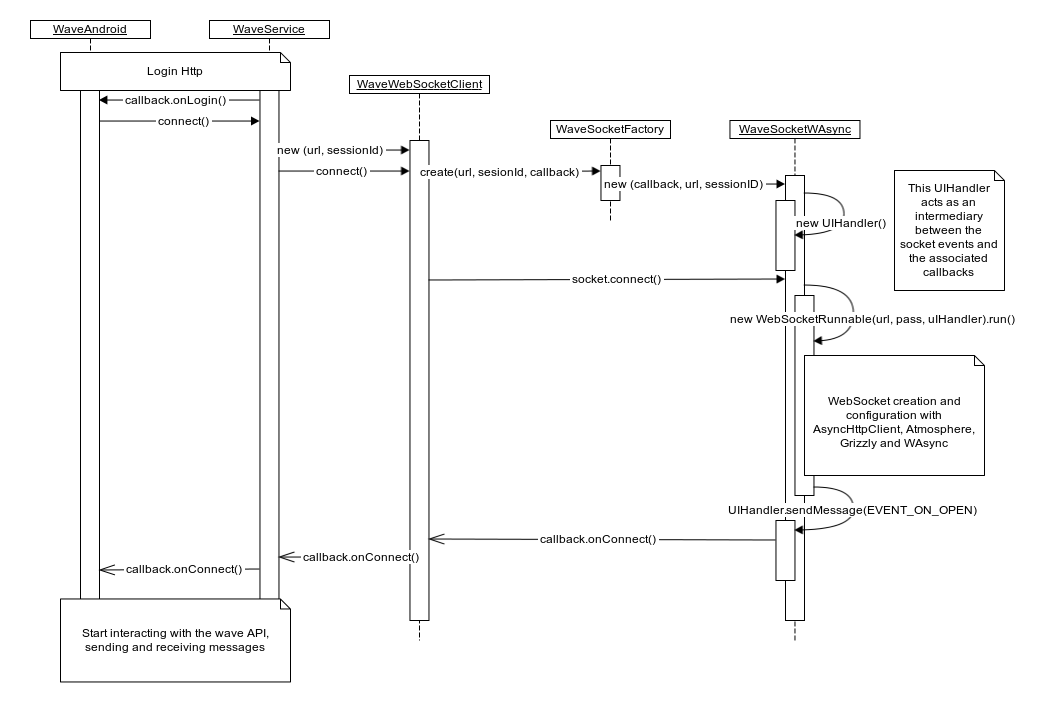
\includegraphics[keepaspectratio, scale=0.43]{Media/Diagrams/waveServerConnectionSequenceDiagram.png}
    \caption{Proceso de conexión WebSocket con Servicio}
   \label{fig:sequenceDiagram_waveWebSocket}
  \end{figure}
     
      Cuando se realiza esta conexión al Servidor Wave, la Actividad es notificada de ello mediante la propagación de callbacks onConnect() que informan del éxito de la conexión. A partir de este momento el socket informará de la misma forma (mediante el envío de mensajes al UIHandler) de otros eventos que se produzcan, ya sea la recepción de datos o la desconexión por ejemplo. De la misma forma la aplicación podrá enviar datos al servidor, ya que el socket se mantiene en el Servicio. 
      
        \begin{figure}[!]
   \centering
	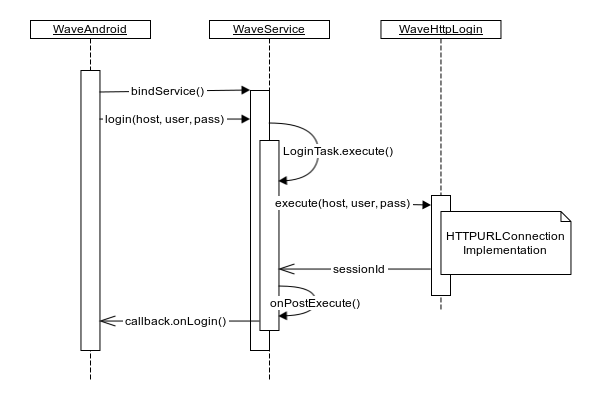
\includegraphics[keepaspectratio, scale=0.6]{Media/Diagrams/loginHttpSequenceDiagram.png}
    \caption{Proceso de conexión Http con Servicio}
   \label{fig:sequenceDiagram_waveHttp}
  \end{figure}
      
    \subsection{Dependencias}
    
    El cliente Android de SwellRT migrado y desarrollado en esta parte del proyecto hace uso de las siguientes dependencias con librerías externas a Android:

    \begin{table}[h]
      \footnotesize
      \begin{center}
	\begin{tabular}{ | c | c | m{8cm} | }
	  \hline
	  \textbf{Nombre} & \textbf{Versión} & \textbf{Descripción} \\
	  \hline
	  WAsync \cite{ref:wAsync_github} & 1.4.3 & Librería que contiene el cliente WebSockets/HTTP para comunicación asíncrona. \\ 
	  \hline
	  AsyncHttpClient \cite{ref:asyncHttpClient} & 1.8.14 & Librería que permite a aplicaciones Java ejecutar de forma sencilla peticiones HTTP y procesar de forma asíncrona la respuesta HTTP recibida. \\ 
	  \hline
	  Grizzly-Framework \cite{ref:grizzly} & \multirow{3}{*}{2.3.18} & Framework del núcleo para aplicaciones Grizzly que proporciona conexiones TCP/UDP, gestión de memoria, servicios/buffers, eventos NIO de bucle/cadenas de filtro/filtros \\ \cline{1-1} \cline{3-3} 
	  Grizzly-Http \cite{ref:grizzly} & & Framework HTTP que contiene la lógica para el tratamiento de mensajes HTTP en el servidor y en el cliente. \\ 
	  \cline{1-1} \cline{3-3} 
	  Grizzly-WebSockets \cite{ref:grizzly} & & Websocket API que permite crear aplicaciones con WebSockets en el servidor y en el cliente. \\ 
	  \hline
	  slf4j-Android \cite{ref:slf4j_android} & 1.6.1 & ''Simple Logging Facade for Java'': Framework de \textit{logging} compatible con Android. \\ 
	  \hline
	\end{tabular}
      \end{center}
      \caption{Dependencias de SwellRT-Android}
      \label{fig:dependencies_swellRT}
    \end{table}       
       
    \subsection{Resultado de la Migración} \label{ssec:migrationResult}
    
    Después de todos estos pasos se dsponía de una versión funcional de SwellRT capaz de conectarse al servidor WIAB de forma nativa desde Android. \textbf{El resultado de esto se puede ver en el GitHub de esta parte del proyecto}\cite{ref:wave_migration_github}.
    
  \begin{figure}[!]
   \centering
	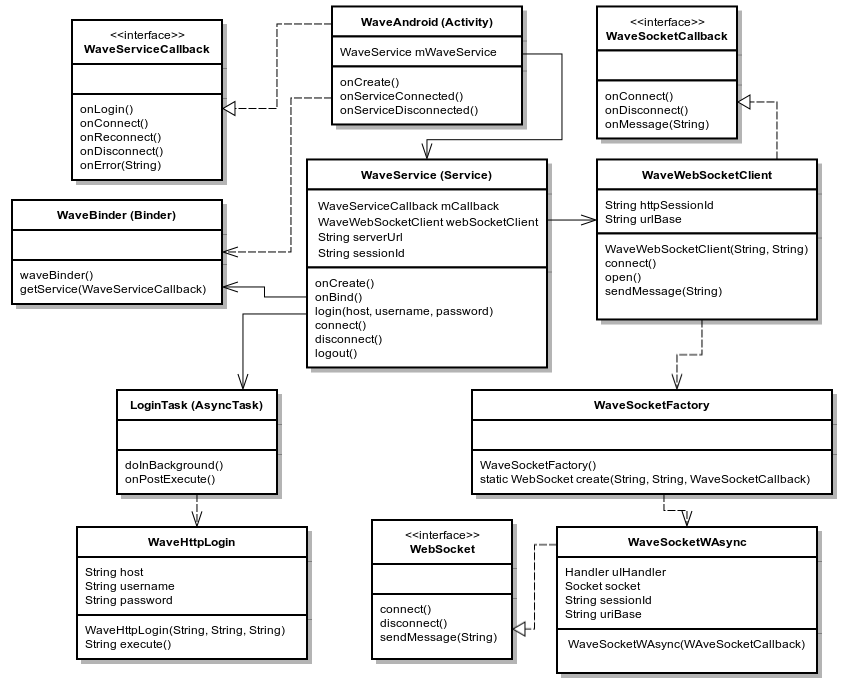
\includegraphics[keepaspectratio, scale=0.5]{Media/Diagrams/waveServiceClassDiagram.png}
    \caption{Esquema de Clases de SwellRT-Android con Servicio}
   \label{fig:sequenceDiagram_waveWebSocket}
  \end{figure}
    
    Solo restaba poner el API de SwellRT en una capa superior para poder acceder y trabajar a nivel de wave con el modelo de datos de SwellRT. De esto se encargó el director de proyecto Pablo, desarrollador del proyecto inicial Web de SwellRT. Con este API trabajaremos en la siguiente parte del proyecto para crear una aplicación Android que haga uso de las funcionalidades de SwellRT. El API se encuentra en el GitHub de SwellRT.
    
    El trabajo realizado para hacer compatible la tecnología de colaboración en tiempo real de Wave presente en SwellRT con dispositivos Android, aporta por primera vez la posibilidad de utilizar estas características de forma nativa en Android en un API de software libre. Hasta este momento las soluciones disponibles pasaban por utilizar librerías privativas como la de Google (Real Time API). Esta nueva aportación se encuentra ahora disponible para los desarrolladores de Android en el GitHub del proyecto de SwellRT: \url{https://github.com/P2Pvalue/swellrt/tree/master/android}

Es además plenamente compatible con el cliente web, por lo que las posibilidades de desarrollo de aplicaciones multi-plataforma son claras. Además, en este proyecto se ha optado por realizar una pequeña prueba de concepto con edición de texto en tiempo real, pero el desarrollo de plataformas colaborativas en tiempo real va más allá e incluye aplicaciones tan diversas como herramientas de dibujo, visualizado de contenidos (como vídeo y música) de forma sincronizada, mapas con información en tiempo real, generación de estadísticas en tiempo real, ...

En definitiva, \textbf{se ha puesto la colaboración en tiempo real a disposición de la comunidad de desarrolladores de Software libre Android para que hagan uso de estas funcionalidades en sus futuras aplicaciones}.